\chapter{ディラックの海、フェルミオン質量、四成分スピノル}

\section{右へ進むフェルミオンとディラックの海}

ディラック方程式はフェルミオンに対する方程式である。相対論的ボソンは、クライン--ゴルドン方程式やマクスウェル方程式など、別の方程式を満たす。最も単純な例は空間一次元に存在し、当初は右にしか進めない粒子と反粒子を記述する。

平面波から始める。
\begin{equation}
\psi(x,t)=\psi_0 e^{i(kx-\omega t)}.
\end{equation}
その位相速度は
\begin{equation}
v_{\mathrm{ph}}=\frac{\omega}{k}.
\end{equation}
である。\(k\) と \(\omega\) の符号が重要である。両者が同符号なら位相は右へ進み、逆符号なら左へ進む。\(\omega\) が \(k\) に比例するとき、位相速度と群速度は一致する。
\begin{equation}
v_{\mathrm{g}}=\frac{d\omega}{dk}=\frac{\omega}{k}.
\end{equation}

一階方程式
\begin{equation}
\frac{\partial\psi}{\partial x}
+
\frac{\partial\psi}{\partial t}
=0.
\end{equation}
を考える。平面波を代入すると
\begin{equation}
ik\psi-i\omega\psi=0,
\end{equation}
となり、したがって
\begin{equation}
\omega=k.
\end{equation}
である。よって波は右へ進む。それに応じて場にラベルを付けると便利である。
\begin{equation}
\frac{\partial\psi_R}{\partial t}
=
-\frac{\partial\psi_R}{\partial x}.
\end{equation}

光速を復元すると次元をもつ形
\begin{equation}
\frac{\partial\psi_R}{\partial x}
+
\frac{1}{c}\frac{\partial\psi_R}{\partial t}
=0,
\end{equation}
が得られ、したがって
\begin{equation}
\omega=ck.
\end{equation}
となる。以後 \(c=1\) とする。\(\hbar=1\) のとき、\(\omega\) は一量子のエネルギーでもある。

\begin{figure}[htbp]
\centering
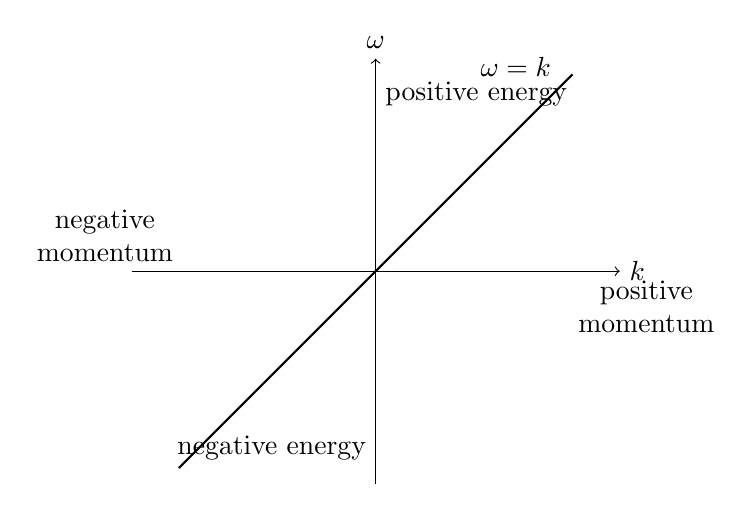
\begin{tikzpicture}[scale=1.0]
\draw[->] (-3.1,0) -- (3.1,0) node[right] {$k$};
\draw[->] (0,-2.7) -- (0,2.7) node[above] {$\omega$};
\draw[thick] (-2.5,-2.5) -- (2.5,2.5);
\node[above left] at (2.35,2.35) {$\omega=k$};
\node[below right,align=center] at (2.45,0) {positive\\momentum};
\node[above left,align=center] at (-2.45,0) {negative\\momentum};
\node[right] at (0,2.25) {positive energy};
\node[left] at (0,-2.25) {negative energy};
\end{tikzpicture}
\caption{質量ゼロの右へ進む分散関係 \(\omega=k\) は正エネルギー枝と負エネルギー枝を含む。}
\end{figure}

この直線には重大な帰結がある。正の \(k\) は正エネルギーを与え、負の \(k\) は負エネルギーを与える。それでも両方の部分は右へ進む波を記述する。なぜなら、全直線上で \(\omega/k=1\) だからである。

正エネルギー部分に置かれた電子は、より低い状態へ落ち、正エネルギーの光子を放出し、また落ち、スペクトルを下り続けることができる。一段下り、また一段、さらに一段と。安定な電子は存在しないことになる。さらに深刻なことに、世界は負エネルギーの電子を次々と生成してエネルギーを下げてしまう。

フェルミオンの排他性が救いを与える。すべての負エネルギー電子状態を埋めるのである。すでに占有された状態へ第二の電子は入れないため、完全に満たされた負エネルギー領域は無限の落下を妨げる。この満たされた領域がディラックの海であり、その完全に満たされた状態が基底状態、すなわち真空である。

\begin{classroomqa}
\lecturetimestamp{00:07:19}
\audiencequestion{さらに低い負エネルギー状態は無限に存在するのか。}
\lecturerresponse{はい。運動量が離散的ならスペクトルは無限のはしごのようであり、運動量が連続的なら連続的な滑り台のようである。負エネルギーの海を埋めることで、電子が無限に下降することは防がれる。ただし、空のより低い状態が利用可能なときには、光子放出を伴う有限の下方遷移が依然として可能でありうる。}
\end{classroomqa}

このことは、このスペクトルをもつ方程式がフェルミオン理論として量子化されなければならない理由を説明する。量子がボソンであれば、任意個の量子が同じ低い状態を占有でき、負エネルギー領域を埋めても真空は安定化しない。

満たされた海の描像は反粒子も生み出す。真空中ではすべての負エネルギー準位が占有され、すべての正エネルギー準位が空である。電子は任意の占有された負エネルギー準位から任意の空の正エネルギー準位へ励起されうる。始状態と終状態の準位は対称に配置される必要はない。

\begin{figure}[htbp]
\centering
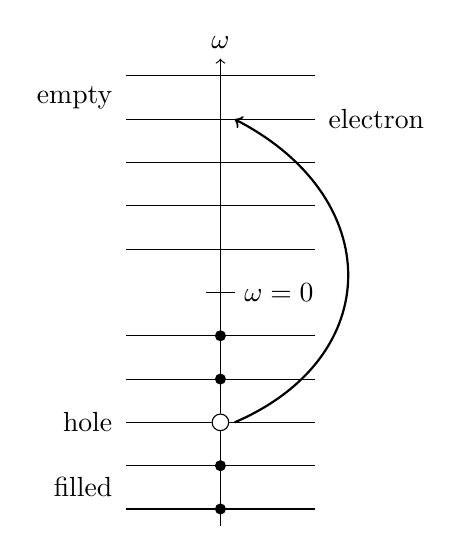
\begin{tikzpicture}[x=1cm,y=0.55cm]
\draw[->] (0,-5.4) -- (0,5.4) node[above] {$\omega$};
\draw (-0.18,0) -- (0.18,0) node[right] {$\omega=0$};
\foreach \y in {-5,-4,-3,-2,-1} {
  \draw (-1.2,\y) -- (1.2,\y);
  \fill (0,\y) circle (2pt);
}
\foreach \y in {1,2,3,4,5} {
  \draw (-1.2,\y) -- (1.2,\y);
}
\draw[->,thick] (0.18,-3) .. controls (2.1,-1.5) and (2.1,2.2) .. (0.18,4);
\draw[white,fill=white] (0,-3) circle (3pt);
\draw (0,-3) circle (3pt);
\node[left] at (-1.25,-3) {hole};
\node[left] at (-1.25,-4.5) {filled};
\node[left] at (-1.25,4.5) {empty};
\node[right] at (1.25,4) {electron};
\end{tikzpicture}
\caption{占有された負エネルギー電子を励起すると、正エネルギーの電子が生じ、満たされた海に空孔が残る。}
\end{figure}

負エネルギーの電子を取り除くと、真空に対してエネルギーが上がるので、空孔は正のエネルギーをもつ。枝 \(\omega=k\) 上では、取り除かれた電子は負の運動量ももっていた。負の運動量を取り除くと正の運動量の超過が残るので、空孔は正の運動量をもつ。電子の電荷を負とすると、失われた電子は正の電荷をもつ。したがって空孔は正エネルギー、正運動量の反粒子であり、励起された電子は負の電荷、正のエネルギー、正の運動量をもつ。この一枝理論におけるすべての実励起は右へ進む。

場 \(\psi_R\) はフェルミオン的生成消滅演算子から構成される。したがって粒子と空孔の解釈は、古典的な波についてだけでなく、場によって生成され消滅させられる量子についての主張である。

依然として非対称性がある。右へ進む海は負の運動量をもつ負エネルギー状態を含む。その形式的な全運動量は巨大で、左を向いている。その定数を差し引くことで真空の運動量をゼロと定義してもよいが、状態は構造的に不均衡なままである。粒子と反粒子は右にしか進まない一方、満たされた真空は負の運動量状態から作られている。

\section{左へ進む枝と釣り合った真空}

左右の釣り合いには、独自の生成消滅演算子をもつ第二の独立な場が必要である。それが次を満たすとしよう。
\begin{equation}
\frac{\partial\psi_L}{\partial t}
=
+\frac{\partial\psi_L}{\partial x}.
\end{equation}
同じ平面波の形に対して、
\begin{equation}
-i\omega\psi_L=ik\psi_L,
\end{equation}
したがって
\begin{equation}
\omega=-k.
\end{equation}
この第二の式は\(\omega=k\)の鏡像である。その正エネルギー分枝は左向きに動く粒子を記述し、その負エネルギー分枝もまた埋められなければならない。

\begin{figure}[htbp]
\centering
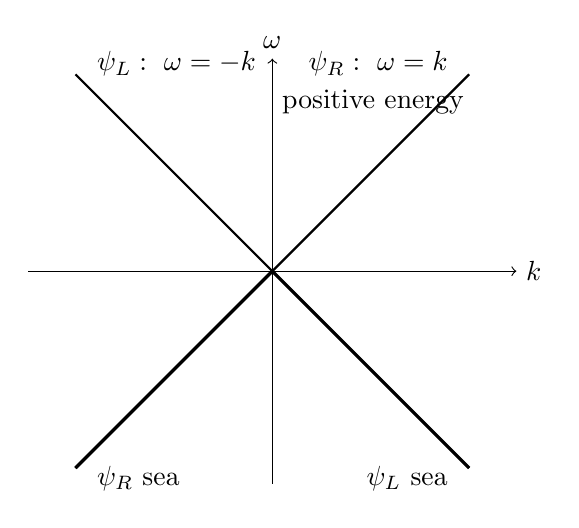
\begin{tikzpicture}[scale=1.0]
\draw[->] (-3.1,0) -- (3.1,0) node[right] {$k$};
\draw[->] (0,-2.7) -- (0,2.7) node[above] {$\omega$};
\draw[thick] (-2.5,-2.5) -- (2.5,2.5);
\draw[thick] (-2.5,2.5) -- (2.5,-2.5);
\draw[very thick] (-2.5,-2.5) -- (0,0);
\draw[very thick] (0,0) -- (2.5,-2.5);
\node[above left] at (2.35,2.35) {$\psi_R:\ \omega=k$};
\node[above right] at (-2.35,2.35) {$\psi_L:\ \omega=-k$};
\node[right] at (0,2.15) {positive energy};
\node[below right] at (-2.35,-2.35) {$\psi_R$ sea};
\node[below left] at (2.35,-2.35) {$\psi_L$ sea};
\end{tikzpicture}
\caption{独立な右向きおよび左向きの場は鏡映された質量ゼロの分枝を与え、二つの負エネルギーの半分の分枝は真空において埋められている。}
\end{figure}

両方の負エネルギー海を埋めた後では、左向きに動く占有状態と右向きに動く占有状態が同数ある。それらの真空運動量は釣り合っている。粒子励起と正孔励起は今やどちらの方向にも動くことができる。

\begin{classroomqa}
\lecturetimestamp{00:15:58}
\audiencequestion{負エネルギーの問題は、埋められた状態と正孔を仮定することなく扱えるだろうか。}
\lecturerresponse{同じ理論は付け替え可能である。埋められた負エネルギーの電子状態を空の反粒子状態と呼んでもよい。そうすれば、物理的な言語には正エネルギーの粒子と反粒子だけが含まれる。埋められた海の描像は、金属における埋められたバンドのように、電子を取り除くと正孔が生じ、励起すると粒子と正孔の両方が生じるという、有用な整合性の検査であり続ける。}
\end{classroomqa}

これまでに考察した励起は質量ゼロである。それらの分散関係は線形であり、その速度の大きさは\(1\)であるから、光速で動く。次の問題は、それらにどのように質量を与えるかである。

\section{二つの成分と質量項}

まず二つの場を一つの列にまとめる。
\begin{equation}
\Psi=
\begin{pmatrix}
\psi_R\\
\psi_L
\end{pmatrix}.
\end{equation}
これは当初、二つの独立な方程式のための簡潔な記法にすぎない。次を定義する。
\begin{equation}
\alpha=
\begin{pmatrix}
1&0\\
0&-1
\end{pmatrix}.
\end{equation}
すると、右向きおよび左向きの方程式は次になる。
\begin{equation}
\frac{\partial\Psi}{\partial t}
=
-\alpha\frac{\partial\Psi}{\partial x}.
\end{equation}

\begin{figure}[htbp]
\centering
\includegraphics[width=0.78\textwidth]{lecture_06_figure_02.png}
\caption{場\(\psi_R\)と\(\psi_L\)は二成分スピノルをなし、\(\alpha\)が二つの質量ゼロの分枝を区別する。}
\lectureframe{00:20:36}
\end{figure}

平面波に対して、演算子
\begin{equation}
i\partial_t
\quad\hbox{and}\quad
-i\partial_x
\end{equation}
はそれぞれ\(\omega\)と\(k\)を返す。したがって行列方程式は次のように略記できる。
\begin{equation}
\omega=\alpha k.
\end{equation}
上側の成分に対してこれは\(\omega=k\)を意味し、下側の成分に対しては\(\omega=-k\)を意味する。この記法は二つの方程式を圧縮したが、新しい物理を持ち込んではいない。

電子は質量ゼロではなく、光速では動かない。そのエネルギーに対する魅力的な式は非相対論的運動エネルギー\(k^2/(2m)\)であるが、それはここでの出発点にはできない。質量ゼロの極限がすでに光速での運動に関わっているからである。相対論的関係は
\begin{equation}
\omega^2=k^2+m^2,
\end{equation}
であり、あるいは両方のエネルギー分枝を含めれば
\begin{equation}
\omega=\pm\sqrt{k^2+m^2}.
\end{equation}
である。\(m=0\)のとき、これらは\(\omega=k\)と\(\omega=-k\)に帰着する。

\begin{classroomqa}
\lecturetimestamp{00:25:23}
\audiencequestion{\(c=1\)となる単位が用いられているのか、また質量をもつ粒子の速さはどのように得られるのか。}
\lecturerresponse{はい。波束の速さは群速度であり、正エネルギー分枝では\(v_{\mathrm g}=d\omega/dk=k/\sqrt{k^2+m^2}\)である。したがって、分散関係そのものが、質量をもつ粒子に対して速さが\(c=1\)より小さくなることを含んでいる。}
\end{classroomqa}

\begin{classroomqa}
\lecturetimestamp{00:26:29}
\audiencequestion{簡略記法\(\omega=\alpha k\)において、\(\omega\)はベクトルか行列か。}
\lecturerresponse{この簡略記法は、二成分波動関数に作用する演算子方程式を表している。ここで\(\omega\)は\(i\partial_t\)を意味し、\(k\)は\(-i\partial_x\)を意味し、\(\alpha\)は成分指数に作用する行列である。スカラー記号\(\omega\)と\(k\)がそれらの数値的な固有値になるのは、平面波においてのみである。}
\end{classroomqa}

方程式を一次のまま保ち、最も単純な質量依存の拡張を試みる。
\begin{equation}
\omega=\alpha k+\beta m.
\end{equation}
対象\(\beta\)は、\(\alpha\)と同じ二成分場に作用するので、行列でなければならない。その代数は二乗することから従う。
\begin{align}
\omega^2
&=(\alpha k+\beta m)(\alpha k+\beta m)\\
&=\alpha^2k^2+\beta^2m^2
+\alpha\beta\,km+\beta\alpha\,mk\\
&=\alpha^2k^2+\beta^2m^2
+(\alpha\beta+\beta\alpha)km.
\end{align}
すべての\(k\)と\(m\)に対して\(k^2+m^2\)を得るには、次を要求する。
\begin{equation}
\alpha^2=I,
\qquad
\beta^2=I,
\qquad
\alpha\beta+\beta\alpha=0.
\end{equation}

二つの通常の非零の数は最後の条件を満たすことができない。数の場合、それは\(2\alpha\beta=0\)を与え、両方の二乗が\(1\)であることに反する。行列は反交換できる。特に、\(\beta\)は\(\alpha\)に等しくなりえない。なぜならそのとき
\begin{equation}
\alpha\beta+\beta\alpha=2\alpha^2=2I.
\end{equation}
となるからである。

次を選ぶ。
\begin{equation}
\beta=
\begin{pmatrix}
0&1\\
1&0
\end{pmatrix}.
\end{equation}
その二乗は成分ごとに確かめられる。
\begin{equation}
\begin{aligned}
\beta^2
&=
\begin{pmatrix}
0&1\\
1&0
\end{pmatrix}
\begin{pmatrix}
0&1\\
1&0
\end{pmatrix}\\
&=
\begin{pmatrix}
0\cdot0+1\cdot1&0\cdot1+1\cdot0\\
1\cdot0+0\cdot1&1\cdot1+0\cdot0
\end{pmatrix}
=
\begin{pmatrix}
1&0\\
0&1
\end{pmatrix}.
\end{aligned}
\end{equation}
乗法の順序が重要である。
\begin{align}
\alpha\beta
&=
\begin{pmatrix}
1&0\\
0&-1
\end{pmatrix}
\begin{pmatrix}
0&1\\
1&0
\end{pmatrix}
=
\begin{pmatrix}
0&1\\
-1&0
\end{pmatrix},\\
\beta\alpha
&=
\begin{pmatrix}
0&1\\
1&0
\end{pmatrix}
\begin{pmatrix}
1&0\\
0&-1
\end{pmatrix}
=
\begin{pmatrix}
0&-1\\
1&0
\end{pmatrix}.
\end{align}
したがって
\begin{equation}
\alpha\beta=-\beta\alpha,
\qquad
\alpha\beta+\beta\alpha=0.
\end{equation}
他の等価な行列の選択も可能であるが、これにより成分方程式が特に透明になる。

微分演算子を戻すと、質量をもつ方程式
\begin{equation}
i\frac{\partial\Psi}{\partial t}
=
-i\alpha\frac{\partial\Psi}{\partial x}
+m\beta\Psi.
\end{equation}
が得られる。行列\(\beta\)は二つの成分を入れ替える。
\begin{equation}
\beta
\begin{pmatrix}
\psi_R\\
\psi_L
\end{pmatrix}
=
\begin{pmatrix}
\psi_L\\
\psi_R
\end{pmatrix}.
\end{equation}
したがって、
\begin{align}
i\dot{\psi}_R
&=-i\frac{\partial\psi_R}{\partial x}+m\psi_L,\\
i\dot{\psi}_L
&=+i\frac{\partial\psi_L}{\partial x}+m\psi_R.
\end{align}

質量項は、質量のない理論では独立していた場を結合する。上側成分の方程式には下側成分が現れ、下側成分の方程式には上側成分が現れる。この結合こそがディラック質量の意味である。方程式は並進不変であるため運動量を保存し、その粒子励起の質量は\(m\)である。

\begin{classroomqa}
\lecturetimestamp{00:38:25}
\audiencequestion{解は自動的にローレンツ不変だろうか？}
\lecturerresponse{特定の解はローレンツ変換の下で固定されたままであるべきではない。一つの運動量をもつ状態は変換された運動量をもつ状態へ移されるので、適切な言い方は共変性である。関係\(\omega^2=k^2+m^2\)はローレンツ不変性の重要な検査の一つであるが、完全な共変性にはスピノル\(\Psi\)の変換則も必要であり、それはまだ確立されていない。}
\end{classroomqa}

\section{静止系と成分の意味}

質量のない粒子は静止させることはできないが、質量をもつ粒子は静止させることができる。静止時には\(k=0\)であるから、波動関数には空間的変化がなく、
\begin{equation}
\omega=\beta m.
\end{equation}
微分方程式は次に帰着する：
\begin{equation}
i\frac{d\Psi}{dt}=m\beta\Psi.
\end{equation}
成分で書くと、
\begin{align}
i\dot{\psi}_R&=m\psi_L,\\
i\dot{\psi}_L&=m\psi_R.
\end{align}
\(\beta\)の非対角成分はどちらも\(+1\)であるから、これらの方程式のいずれにも余分な負号はない。

成分を加えたり引いたりした後、方程式は分離する。次を定義する：
\begin{equation}
\psi_+=\psi_R+\psi_L,
\qquad
\psi_-=\psi_R-\psi_L.
\end{equation}
静止系の二つの方程式を加えると
\begin{equation}
i\dot{\psi}_+=m\psi_+,
\end{equation}
が得られ、引くと
\begin{equation}
i\dot{\psi}_-=-m\psi_-.
\end{equation}
が得られる。したがって
\begin{equation}
\omega=+m
\quad\hbox{for }\psi_+,
\qquad
\omega=-m
\quad\hbox{for }\psi_-.
\end{equation}

\begin{figure}[htbp]
\centering
\includegraphics[width=0.62\textwidth]{lecture_06_figure_03.png}
\caption{運動量がゼロのとき、\(\psi_+=\psi_R+\psi_L\)と\(\psi_-=\psi_R-\psi_L\)は静止振動数\(\omega=+m\)と\(\omega=-m\)をもつ。}
\lectureframe{00:44:49}
\end{figure}

正エネルギーの静止場は\(\psi_+\)であり、負エネルギーの静止場は\(\psi_-\)である。負エネルギー状態は、以前と同様に満たされている。静止系の結果は全スペクトルの\(k=0\)の断面にすぎない：
\begin{equation}
\omega_\pm(k)=\pm\sqrt{k^2+m^2}.
\end{equation}
\begin{figure}[htbp]
\centering
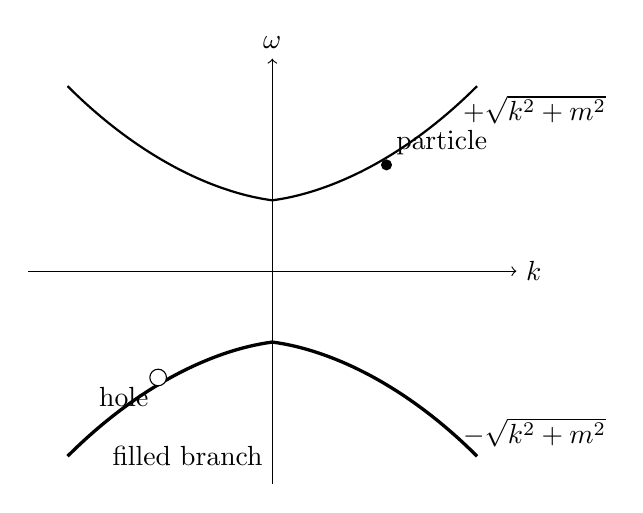
\begin{tikzpicture}[scale=1.0]
\draw[->] (-3.1,0) -- (3.1,0) node[right] {$k$};
\draw[->] (0,-2.7) -- (0,2.7) node[above] {$\omega$};
\draw[thick] (-2.6,2.35)
  .. controls (-1.7,1.45) and (-0.75,1.0) .. (0,0.9)
  .. controls (0.75,1.0) and (1.7,1.45) .. (2.6,2.35);
\draw[very thick] (-2.6,-2.35)
  .. controls (-1.7,-1.45) and (-0.75,-1.0) .. (0,-0.9)
  .. controls (0.75,-1.0) and (1.7,-1.45) .. (2.6,-2.35);
\fill (1.45,1.35) circle (2pt);
\node[above right] at (1.45,1.35) {particle};
\fill[white] (-1.45,-1.35) circle (3pt);
\draw (-1.45,-1.35) circle (3pt);
\node[below left] at (-1.45,-1.35) {hole};
\node[right] at (2.3,2.05) {$+\sqrt{k^2+m^2}$};
\node[right] at (2.3,-2.05) {$-\sqrt{k^2+m^2}$};
\node[left] at (0,-2.35) {filled branch};
\end{tikzpicture}
\caption{どの運動量でも、質量をもつスペクトルには正エネルギー状態と負エネルギー状態がある。負の枝は満たされており、そこに欠けている状態は正エネルギーの空孔である。}
\end{figure}
どの運動量にも正エネルギー状態と負エネルギー状態がある。負の枝のすべての状態を満たすと、海の上には正エネルギーの粒子が、海の中には正エネルギーの空孔が残る。粒子も空孔も正の質量をもつ。

本質的な点は繰り返すに値する。フェルミオンは、以前は独立であった二つの成分が結合されると質量をもつようになる。静止時には、元の成分のどちらも単独ではエネルギー固有状態ではない。確定したエネルギーの状態はそれらの和と差である。

和が何を意味するかを見るために、関連する一粒子生成部分を\(C_R^\dagger\)および\(C_L^\dagger\)と書く。真空に作用すると、
\begin{equation}
(C_R^\dagger+C_L^\dagger)\lvert0\rangle
\end{equation}
は二つの成分のコヒーレントな重ね合わせにある一粒子を生成する。二粒子を生成するのではない。積
\begin{equation}
C_R^\dagger C_L^\dagger\lvert0\rangle,
\end{equation}
は二つの生成演算子を含み、両方のモードが利用可能なとき二粒子状態を生成する。規格化後、静止状態は二つの成分に等しい確率をもつが、結合した波全体としては運動量がゼロである。

ラベル\(R\)と\(L\)は、\(m=0\)のときにのみ文字通りの運動ラベルであった。質量項が存在すると、運動する質量をもつ解は一般に両方の成分を含み、静止解はそれらを等しい大きさで含む。したがって、ここでは\(R\)と\(L\)を上側および下側スピノル成分のラベルとみなす方がよい。

\begin{figure}[htbp]
\centering
\includegraphics[width=0.78\textwidth]{lecture_06_figure_04.png}
\caption{質量が非ゼロの場合、二つのスピノル成分は結合しており、それらの右移動・左移動の解釈は質量のない極限でのみ直接当てはまる。}
\lectureframe{00:50:48}
\end{figure}

素粒子物理学におけるすべての質量をもつフェルミオンは、左成分場と右成分場から構成される。ディラック質量は、質量のない極限では独立である成分を結合する。

\begin{classroomqa}
\lecturetimestamp{00:52:01}
\audiencequestion{\(\psi_R\pm\psi_L\)は\(1/\sqrt{2}\)の因子を含むべきだろうか？}
\lecturerresponse{状態を規格化するために含めてもよい。それは方程式の両辺に掛かるので、運動方程式を変えない。}
\end{classroomqa}

\begin{classroomqa}
\lecturetimestamp{00:52:12}
\audiencequestion{右成分と左成分の相対的な大きさは重要だろうか？}
\lecturerresponse{選ばれた静止系固有状態では、それらの大きさは等しい。全体の規格化は任意であるが、相対的な大きさは\(\beta\)の固有ベクトルによって固定される。}
\end{classroomqa}

\begin{classroomqa}
\lecturetimestamp{00:52:52}
\audiencequestion{二つの成分は相対位相を持ちうるか。}
\lecturerresponse{はい。\(\psi_R\pm\psi_L\)における実係数は、実数である\(\beta\)を選ぶことから従う。二乗すると単位行列となり、\(\alpha\)と反可換となる他の行列も等価な選択であり、その場合には成分間に位相が現れうる。ひとたび表現を選んだならば、それを一貫して用いなければならない。}
\end{classroomqa}

\begin{classroomqa}
\lecturetimestamp{00:53:43}
\audiencequestion{質量が加わった後で``左向き移動成分''および``右向き移動成分''というラベルは誤解を招くか。}
\lecturerresponse{いくらかは。それらは質量ゼロの理論における真の左向きおよび右向きの波を記述する。質量が非零の場合、一方向に運動する粒子でさえ一般には両方の成分を含むので、``上成分''および``下成分''の方が安全なラベルである。}
\end{classroomqa}

\begin{classroomqa}
\lecturetimestamp{00:55:01}
\audiencequestion{静止したフェルミオンはすでにスピン角運動量を必要とするか。}
\lecturerresponse{この一次元模型では必要としない。角運動量は一次元空間では定義されないので、スピンはまだこの構成に現れていない。}
\end{classroomqa}

\begin{classroomqa}
\lecturetimestamp{00:55:24}
\audiencequestion{波動関数はフェルミオン的生成消滅演算子を含むか。}
\lecturerresponse{はい。}
\end{classroomqa}

\begin{classroomqa}
\lecturetimestamp{00:55:30}
\audiencequestion{生成消滅演算子の選択以外に、フェルミオン的性質はどこから入るのか。}
\lecturerresponse{それはフェルミオン的生成--消滅規則を通じて入る。この負エネルギー・スペクトルをもつ方程式はそれらの規則で量子化されなければならない。ボソン的占有規則では真空が不安定なままとなる。相対論的ボソンは別の波動方程式で記述されなければならない。}
\end{classroomqa}

\begin{classroomqa}
\lecturetimestamp{00:56:20}
\audiencequestion{非零運動量の解はローレンツ変換によって静止系の解に移せるか。}
\lecturerresponse{はい。ブーストは質量をもつ解をその静止系へ移せるが、その変換を実行するにはローレンツ変換がスピノル\(\Psi\)にどのように作用するかを知る必要がある。}
\end{classroomqa}

\section{スカラー真空場からの質量}

\begin{classroomqa}
\lecturetimestamp{00:58:11}
\audiencequestion{ヒッグス場との相互作用はどのようにディラック質量項を生じるのか。}
\lecturerresponse{定数の質量係数をスカラー場との結合に置き換える。その場が真空中でゼロならば、フェルミオンは質量ゼロのままである。その場が定数の非零真空値をもつならば、その結合はちょうど質量のように働く。}
\end{classroomqa}

\(\phi(x,t)\)をそれ自身の運動方程式をもつスカラー場とする。ディラック方程式において、質量項の定数\(m\)を\(g\phi(x,t)\)で置き換える：\footnote{表示された相互作用項は、先に確立した質量項\(m\beta\Psi\)でこの置き換えを行うことによって得られる。}
\begin{equation}
i\frac{\partial\Psi}{\partial t}
=
-i\alpha\frac{\partial\Psi}{\partial x}
+g\phi(x,t)\,\beta\Psi.
\end{equation}
すると2つの場の方程式は結合する。フェルミオンはスカラー場に作用し、スカラー場はフェルミオンに作用し返す。合わせて考えると、与えられた\(\phi\)に対してディラック方程式が\(\Psi\)について線形であっても、系は非線形である。

まず、空の空間が
\begin{equation}
\phi(x,t)=0.
\end{equation}
をもつと仮定する。すると混合項は消え、上成分と下成分は分離し、フェルミオンは質量ゼロとなる。代わりに、最低エネルギー状態が定数の非零スカラー場をもつと仮定する：
\begin{equation}
\phi(x,t)=\phi_0\neq0.
\end{equation}
その真空におけるディラック方程式は
\begin{equation}
i\frac{\partial\Psi}{\partial t}
=
-i\alpha\frac{\partial\Psi}{\partial x}
+g\phi_0\,\beta\Psi,
\end{equation}
となるので、
\begin{equation}
m_{\mathrm{eff}}=g\phi_0.
\end{equation}
となる。したがって、ボソン場とフェルミオン場の間の結合と、空の空間におけるボソン場の非零値とが相まって、以前に方程式へ直接書き込まれた質量として現れたのと同じ左右混合を生じる。

\begin{classroomqa}
\lecturetimestamp{01:01:27}
\audiencequestion{LHCは真空中の非零ヒッグス場の証拠を与え得るか。}
\lecturerresponse{もちろん。それは大きな問題の一つである。}
\end{classroomqa}

\begin{classroomqa}
\lecturetimestamp{01:01:32}
\audiencequestion{ヒッグス機構がどのように働くかをもっと話せますか。}
\lecturerresponse{スカラー場はその空間的および時間的変化に伴うエネルギーをもち、また局所的なポテンシャルエネルギー\(V(\phi)\)をもち得る。そのポテンシャルの極小が\(\phi\)の非零値に生じるならば、真空は非零の場を含む。選ばれた極小のまわりの量子化された振動がヒッグス粒子である。}
\end{classroomqa}

場は2つの異なる仕方でエネルギーを担い得る。あるエネルギーは場が空間的および時間的にどのように変化するかに依存する。マクスウェル場はよく知られた比較対象である：
\begin{equation}
\mathcal{E}_{\mathrm{Maxwell}}\propto \mathbf E^2+\mathbf B^2,
\end{equation}
そして\(\mathbf E\)と\(\mathbf B\)の両方は電磁ポテンシャルの微分から作られる。したがってこのエネルギーは、基礎となる場の空間的および時間的変化に伴うものである。

スカラー場はまた、局所的なポテンシャルエネルギー密度
\begin{equation}
V(\phi),
\end{equation}
を持つことができる。これは\(\phi\)自身の値に依存し、その微分には依存しない。模式的には、
\begin{equation}
\mathcal{E}_\phi
=
\mathcal E_{\text{space and time gradients}}+V(\phi).
\end{equation}
となる。これを定めるより深い原理がなければ、\(V(\phi)\)は模型の対称性と両立する任意の妥当な関数であり得る。

ここで用いている単純化された実スカラーの例では、理論が
\begin{equation}
\phi\longrightarrow-\phi.
\end{equation}
の下で対称であるとする。そのときポテンシャルは偶でなければならない：
\begin{equation}
V(\phi)=V(-\phi).
\end{equation}
この対称性だけでは最小値がどこにあるかはわからない。一つの可能性は\(\phi=0\)における単一の最小値である。もう一つは、非零の値における対称な一対の最小値であり、一方は正でもう一方は負である。

\begin{figure}[htbp]
\centering
\includegraphics[width=0.72\textwidth]{lecture_06_figure_05.png}
\caption{\(\phi=0\)における最小値は真空の場を零にするが、対称な非零の最小値は真空値\(\phi_0\neq0\)を許し、したがってフェルミオン質量\(g\phi_0\)を与える。}
\lectureframe{01:04:47}
\end{figure}

この二つの可能性は、ポテンシャルの特定の多項式形にコミットすることなく描くことができる。\footnote{以下の曲線は、議論で用いた定性的な中心最小値と対称性に関連する最小値のみを保っている。}
\begin{figure}[htbp]
\centering
\resizebox{\linewidth}{!}{%
\begin{tikzpicture}[x=1.35cm,y=1.05cm]
\begin{scope}[shift={(-3.1,0)}]
\draw[->] (-1.7,0) -- (1.7,0) node[right] {$\phi$};
\draw[->] (0,-0.15) -- (0,2.45) node[above] {$V(\phi)$};
\draw[thick] (-1.5,2.05) .. controls (-0.9,0.65) and (-0.45,0.25) .. (0,0.25)
             .. controls (0.45,0.25) and (0.9,0.65) .. (1.5,2.05);
\fill (0,0.25) circle (1.2pt);
\node[below] at (0,0) {$0$};
\end{scope}
\begin{scope}[shift={(3.1,0)}]
\draw[->] (-1.7,0) -- (1.7,0) node[right] {$\phi$};
\draw[->] (0,-0.15) -- (0,2.45) node[above] {$V(\phi)$};
\draw[thick] (-1.55,2.05)
  .. controls (-1.25,0.75) and (-1.0,0.25) .. (-0.75,0.25)
  .. controls (-0.35,0.25) and (-0.25,1.3) .. (0,1.3)
  .. controls (0.25,1.3) and (0.35,0.25) .. (0.75,0.25)
  .. controls (1.0,0.25) and (1.25,0.75) .. (1.55,2.05);
\fill (-0.75,0.25) circle (1.2pt);
\fill (0.75,0.25) circle (1.2pt);
\node[below] at (0,0) {$0$};
\node[below] at (-0.75,0) {$-\phi_0$};
\node[below] at (0.75,0) {$\phi_0$};
\end{scope}
\end{tikzpicture}%
}
\caption{偶ポテンシャルは中心最小値をもつことも、対称性に関連する二つの非零最小値をもつこともある。}
\end{figure}

最小値が原点にあるなら、真空は\(\phi_0=0\)をもち、この結合は電子に質量を与えない。最小値が\(\phi=\pm\phi_0\)にあるなら、真空はどちらか一方に落ち着く。二つの選択肢は対称性によって関係しており、どちらもディラック方程式に非零の係数\(g\phi_0\)を生じる。なぜポテンシャルがこの定性的な形をとるのかはより深い問題であり、この機構自体によって決着するものではない。

場は正確に最小値にとどまる必要はない。粒子がポテンシャル井戸の底の近くで振動できるのとちょうど同じように、場は選ばれた値のまわりで振動できる。それらの振動を量子化するとヒッグス量子が得られる。その特徴的な振動数はヒッグス粒子の質量と関係する。質量が大きいとは、一つの量子を励起するのにさえ大きなエネルギーが必要であることを意味する。真空中では場は単に最小値の近くにあり、フェルミオン質量を与えている。場が振動するとき、その振動がヒッグス粒子である。

この結合は作用と反作用を伴う。フェルミオンは\(\phi\)の値に応答するが、十分に高エネルギーのフェルミオン衝突はスカラー場を励起することもできる。衝突は励起エネルギーを供給しなければならない。ひとたび場が振動すれば、その量子はヒッグス粒子である。同じ場は電子だけでなく、クォーク場や、その質量をこの場が供給する他の場とも結合する。

\begin{classroomqa}
\lecturetimestamp{01:08:14}
\audiencequestion{ヒッグス場が振動したり変位したりすると、電子の質量は変化するのか。}
\lecturerresponse{はい。有効質量は場の局所的な値に比例するので、場を零の方向へ変位させると質量は減少する。巨視的な領域を真空の値から遠く離れたところに保つには莫大なエネルギーが必要であり、そのような実験に十分な大きさの領域はブラックホールに崩壊しうる。}
\end{classroomqa}

この思考実験は直接的である。もしある領域を\(\phi=0\)の近くに保つことができれば、その領域内では
\begin{equation}
m_{\mathrm{eff}}=g\phi
\end{equation}
が小さくなるか零になる。励起されたヒッグスモードは真空の値のまわりで振動するが、巨視的な領域全体にわたって無視できない変位を生成し維持するには莫大なエネルギーが必要である。ポテンシャルエネルギーの代償は体積とともに増大する。そのような領域が実用的な実験室になるはるか前に、そのエネルギーは重力崩壊を起こすのに十分なほど大きくなりうる。質量の変化は原理的には実在するが、大きな観測可能な変化を実現するのは途方もなく困難である。

\begin{classroomqa}
\lecturetimestamp{01:09:27}
\audiencequestion{なぜヒッグス場が必要なのか。}
\lecturerresponse{電子が質量をもつからである。}
\end{classroomqa}

\begin{classroomqa}
\lecturetimestamp{01:09:41}
\audiencequestion{粒子の種類ごとにそれぞれのヒッグス場があるのか。}
\lecturerresponse{いいえ。標準模型では一つのヒッグス場が、電子、クォーク、およびこの機構に関与する他の粒子に質量を供給する。超対称版では、粒子種ごとに別々の場が一つずつ必要になるのではなく、二つのヒッグス場が必要である。}
\end{classroomqa}

一つの場という描像は概略的である。完全なヒッグス場は単一の実数\(\phi\)よりも多くの構造をもつ。それでも本質的な点は生き残る。共通の真空の場が異なるフェルミオンと異なる強さで結合しうるので、異なる質量のために粒子種ごとに異なるヒッグス場が必要なわけではない。ヒッグス粒子は、その同じ場がその真空値のまわりで振動するものである。

なぜ単に電子の質量を手で方程式に入れてヒッグス場を不要にしないのか。その答えは弱い相互作用と統一に関係しており、後回しにする。

\begin{classroomqa}
\lecturetimestamp{01:11:16}
\audiencequestion{超対称性理論では、ヒッグスセクターは2つあるのか。}
\lecturerresponse{はい。ここで用いている簡略化された区分では、一方がアップ型クォークに質量を与え、他方がダウン型クォークと電子に質量を与える。この二重化は超対称性の技術的要請であり、粒子ごとに別個のヒッグス場があるわけではない。}
\end{classroomqa}

\begin{classroomqa}
\lecturetimestamp{01:12:01}
\audiencequestion{ヒッグス粒子に質量があるなら、その質量はどこから来るのか。}
\lecturerresponse{その問いはここでは解決されない。より鋭い謎は、なぜヒッグス質量がそれほど小さいのかということである。}
\end{classroomqa}

対称性は質量の問題と切り離せない。単純なディラック模型では、左セクターと右セクターが混合するのを妨げる対称性があれば、混合項の係数はゼロになる。真空がその対称性を尊重していれば、フェルミオンは質量をもたない。ヒッグス真空期待値がゼロでないことが、関連する真空の対称性を破り、左右の結合を可能にする：
\begin{equation}
m_{\mathrm{eff}}=g\phi_0\neq0.
\end{equation}
正確な対称性変換はここでは展開しない。要点は質量項に対するその帰結である。方程式はその対称性をもちうるが、特定の最低エネルギー状態はそうではない。質量を与えるのは、この真空の非対称性である。

ここで概説している電弱の描像では、電子とクォークはこのようにして質量を獲得し、\(W\)ボソンと\(Z\)ボソンも同様である。光子は質量のないままである。ヒッグス粒子自身はもう一つの例外である。それは同じ真空の変位がなくても質量をもちうるし、その質量は左右のフェルミオン混合ではなく、自身の場の振動に関わる。したがって、ヒッグス真空期待値はこの説明における他の粒子の質量を生み出す一方、ヒッグス励起の質量は別個の問いを提起する。

\begin{classroomqa}
\lecturetimestamp{01:15:26}
\audiencequestion{重力子には質量があるのか。}
\lecturerresponse{いいえ。重力子は光子と同様、質量をもたない。ニュートリノもかつては質量をもたないと考えられていたが、非常に小さな質量をもつ。現在の言葉でいえば、その左成分と右成分の結合がごくわずかであるということである。}
\end{classroomqa}

光子と、理論における重力子は質量をもたず、光速で運動する。ニュートリノはまったくそのクラスに属するわけではない。その微小な質量は、このディラックの言葉では、左成分と右成分を結びつける結合が微小であることを意味する。なぜそれがそれほど小さいのかは、また別の問いである。

\section{3次元空間におけるディラック方程式}

3次元空間では、波数は波数ベクトルになる：
\begin{equation}
\mathbf{k}=(k_1,k_2,k_3),
\end{equation}
その成分は\(x\)方向、\(y\)方向、\(z\)方向に沿っている。1次元の関係は符号
\begin{equation}
\omega=\alpha k+\beta m,
\end{equation}
をもち、その最も単純な線形一般化は
\begin{equation}
\omega
=
\alpha_1 k_1+\alpha_2 k_2+\alpha_3 k_3+\beta m.
\end{equation}
である。ここで\(\alpha_i\)と\(\beta\)は行列である。それらは
\begin{equation}
\omega^2=k_1^2+k_2^2+k_3^2+m^2.
\end{equation}
となるように選ばれなければならない。この不変な分散関係は本質的な条件であるが、それ自体では相対性理論の内容のすべてではない。

線形表現を二乗すると
\begin{align}
\omega^2
={}&
\alpha_1^2k_1^2+\alpha_2^2k_2^2+\alpha_3^2k_3^2+\beta^2m^2
\nonumber\\
&+(\alpha_1\alpha_2+\alpha_2\alpha_1)k_1k_2
+(\alpha_1\alpha_3+\alpha_3\alpha_1)k_1k_3
\nonumber\\
&+(\alpha_2\alpha_3+\alpha_3\alpha_2)k_2k_3
+\sum_{i=1}^{3}(\alpha_i\beta+\beta\alpha_i)k_i m.
\end{align}
となる。二乗された運動量の係数と質量は
\begin{equation}
\alpha_1^2=\alpha_2^2=\alpha_3^2=I,
\qquad
\beta^2=I.
\end{equation}
を要求する。不要な\(k_i k_j\)項は、異なる\(\alpha\)行列が反可換ならば消える：
\begin{equation}
\alpha_i\alpha_j+\alpha_j\alpha_i=0,
\qquad i\neq j.
\end{equation}
混合した\(k_i m\)項は、
\begin{equation}
\alpha_i\beta+\beta\alpha_i=0
\qquad
\text{for each }i.
\end{equation}
ならば消える。したがって、4つの行列はすべて単位行列に二乗され、異なる行列のどの対も反可換である。

必要な相互反可換性の性質をもつ3つの\(2\times2\)行列は実際に存在する。それらは3つのパウリ行列である。単位行列に二乗され、かつ3つすべてと反可換する4番目の\(2\times2\)行列は存在しない。\(3\times3\)の実現もどれもうまくいかない。最初に可能な実現は\(4\times4\)行列、すなわちディラック行列を用いる。

2成分から4成分への移行は物理的な問いを提起する。1次元空間では、2つの成分は右進行場と左進行場として始まった。4つの成分は何を意味するのか。新しい要素はスピンになるが、スピンは角運動量を必要とし、したがって真に3次元の議論を必要とする。

行列は一意ではない。異なる選択は、互いに直交する座標軸の異なる選択が等価であるのとほぼ同じ意味で等価である。成分は変わるが、変換が記述を関係づけ、物理は変わらない。便利な表現の一つは\footnote{以下に示す成分ごとの行列は、その直後に示すブロック形式とパウリ行列の展開である。それらのブロック関係は01：30：23--01：31：29の講義で明示的に述べられている。}
\begin{equation}
\beta=
\begin{pmatrix}
1&0&0&0\\
0&1&0&0\\
0&0&-1&0\\
0&0&0&-1
\end{pmatrix},
\end{equation}
および
\begin{align}
\alpha_1&=
\begin{pmatrix}
0&0&0&1\\
0&0&1&0\\
0&1&0&0\\
1&0&0&0
\end{pmatrix},
&
\alpha_2&=
\begin{pmatrix}
0&0&0&-i\\
0&0&i&0\\
0&-i&0&0\\
i&0&0&0
\end{pmatrix},
\\[1ex]
\alpha_3&=
\begin{pmatrix}
0&0&1&0\\
0&0&0&-1\\
1&0&0&0\\
0&-1&0&0
\end{pmatrix}.
\end{align}
とともに。それらの構造は、各行列を\(2\times2\)ブロックに分けると見やすい：
\begin{equation}
\beta=
\begin{pmatrix}
I_2&0\\
0&-I_2
\end{pmatrix},
\qquad
\alpha_i=
\begin{pmatrix}
0&\sigma_i\\
\sigma_i&0
\end{pmatrix}.
\end{equation}
3つのパウリ行列は
\begin{equation}
\sigma_1=
\begin{pmatrix}
0&1\\
1&0
\end{pmatrix},
\quad
\sigma_2=
\begin{pmatrix}
0&-i\\
i&0
\end{pmatrix},
\quad
\sigma_3=
\begin{pmatrix}
1&0\\
0&-1
\end{pmatrix}.
\end{equation}
である。これらのブロック行列は要求されるディラック反交換関係を満たす。

波動関数は今や四つの成分を持たなければならない：
\begin{equation}
\Psi=
\begin{pmatrix}
\psi_1\\
\psi_2\\
\psi_3\\
\psi_4
\end{pmatrix}.
\end{equation}
運動方程式は
\begin{equation}
i\frac{\partial\Psi}{\partial t}
=
-i\sum_{j=1}^{3}\alpha_j
\frac{\partial\Psi}{\partial x_j}
+\beta m\Psi.
\end{equation}
この簡潔な表現は四つの連立線形微分方程式を表している。\(\alpha_j\)の非対角成分は、一次元の場合よりも複雑な仕方で四つの成分を混合するが、基本的な構造は同じである。すなわち、行列が成分を結合し、方程式は空間と時間について一次にとどまる。成分がさらに二倍になることが、スピンへと導く手がかりである。

\begin{classroomqa}
\lecturetimestamp{01:33:53}
\audiencequestion{\(\Psi\)の4つの成分は、時空の4つの次元に直接対応する4元ベクトルなのか。}
\lecturerresponse{いいえ。それらは4元ベクトルではなくスピノルをなす。1次元の例で時空の次元の数とスピノルの成分の数が等しかったのは偶然であった。より高次元の構成では、スピノル行列の大きさは2の冪で現れ、一般には時空の次元の数と等しくならない。}
\end{classroomqa}

再び静止系が最も単純な解釈を与える。運動量がゼロのとき、微分項は消える：
\begin{equation}
i\frac{\partial\Psi}{\partial t}=m\beta\Psi.
\end{equation}
選んだ表現において、\(\beta\)は二つの固有値\(+1\)と二つの固有値\(-1\)を持つ。したがって、エネルギー\(+m\)を持つ二つの静止状態と、エネルギー\(-m\)を持つ二つの静止状態が存在する。以前と同様に、負エネルギーの状態は満たされている。各エネルギー符号内の二重の多重度が、その物理的解釈がスピンである余分な構造である。

\begin{classroomqa}
\lecturetimestamp{01:35:51}
\audiencequestion{\(\alpha_i\)の非対角ブロックは同じ添字をもつべきであり、したがってそれらは\(\sigma_i\)なのか。}
\lecturerresponse{はい。各行列\(\alpha_i\)は、両方の非対角ブロックに対応するパウリ行列\(\sigma_i\)を含む。}
\end{classroomqa}

\begin{classroomqa}
\lecturetimestamp{01:36:03}
\audiencequestion{\(\alpha_i\)の簡潔な反交換関係には因子2が欠けているのか。}
\lecturerresponse{はい。\(i=j\)のとき、左辺は\(\alpha_i^2+\alpha_i^2=2I\)である。正しい関係は\(\alpha_i\alpha_j+\alpha_j\alpha_i=2\delta_{ij}I\)である。}
\end{classroomqa}

したがって、平方の条件と添字が異なる場合の条件を別々に扱ったものを、次のようにまとめることができる：
\begin{equation}
\alpha_i\alpha_j+\alpha_j\alpha_i=2\delta_{ij}I.
\end{equation}

\begin{classroomqa}
\lecturetimestamp{01:36:42}
\audiencequestion{4つの行列への移行は、ディラックの構成における大きな概念的飛躍であったのか。}
\lecturerresponse{はい。ディラックは方程式を仮定し、その帰結を追った。一つの帰結は反粒子の出現であり、もう一つはスピンであった。スピンはすでに経験的に知られていたが、方程式がそれを説明した。}
\end{classroomqa}

\begin{classroomqa}
\lecturetimestamp{01:37:29}
\audiencequestion{粒子をボソンとフェルミオンに限る定理と経験的証拠のどちらが先に来たのか。}
\lecturerresponse{経験的証拠が先に来て、定理は後であった。ボソン--フェルミオンという選択肢は3次元空間で成り立つ。2次元空間と1つの時間次元では、中間的な統計が起こりうる。\(3+1\)次元およびより高い空間次元では、選択肢はボソンとフェルミオンである。}
\end{classroomqa}

\begin{classroomqa}
\lecturetimestamp{01:39:01}
\audiencequestion{\(\Psi\)の4つの成分に慣習的な添字はあるのか。}
\lecturerresponse{ここでは本質的な選択は固定されていない。ラベル\(p\)と\(q\)を用いることができ、1から4まで走る。そのとき各行列は1つの行の添字と1つの列の添字をもつ。}
\end{classroomqa}

行列記法はこれらの成分ラベルを隠す。それらを露わにすれば、
\begin{equation}
p,q=1,2,3,4,
\end{equation}
となり、方程式は次のようになる：
\begin{equation}
i\,\partial_t\Psi_p
=
-i\sum_{j=1}^{3}\sum_{q=1}^{4}
(\alpha_j)_{pq}\,\partial_j\Psi_q
+m\sum_{q=1}^{4}\beta_{pq}\Psi_q.
\end{equation}

\begin{classroomqa}
\lecturetimestamp{01:40:15}
\audiencequestion{行列の掛け算を用いるとき、明示的な成分の添字は不要なのか。}
\lecturerresponse{はい。行列記法はそれらの添字を自動的に隠す。相対論的構造をより明示的にする、より対称的な形は後で導入できる。}
\end{classroomqa}

表示された方程式は、最も単純な\(3+1\)次元の形のディラック方程式である。次の段階は、スピンを理解することと、相対論的ボソンの波動方程式を構成することである。ディラック方程式はそれらの方程式ではなく、自然界の粒子のおよそ半分はボソンだからである。これらの材料が揃えば、クォーク、レプトン、弱ゲージボソン、ヒッグス粒子、光子へと進み、粒子のスペクトルにいくらかの秩序をもたらすことができる。その議論全体を通じて、さらなる対称性が必要である。
